\section{Einführung und Überblick}

\begin{definition}{Software Engineering}
    \begin{itemize}
        \item \textbf{Disziplinen}: \\
        Anforderungen, Architektur, Implementierung, Test und Wartung
        \item \textbf{Ziel}: \\
        Strukturierte Prozesse für Qualität, Risiko- \& Fehlerminimierung
    \end{itemize}
    \end{definition}


\subsubsection{Softwareentwicklungsprozesse}

\begin{concept}{Dimensionen der Softwareentwicklung}
\begin{itemize}
    \item Requirements (Bekannt - Unbekannt)
    \item Technology (Bekannt - Unbekannt)  
    \item Skills/Experience (Vorhanden - Nicht vorhanden)
\end{itemize}
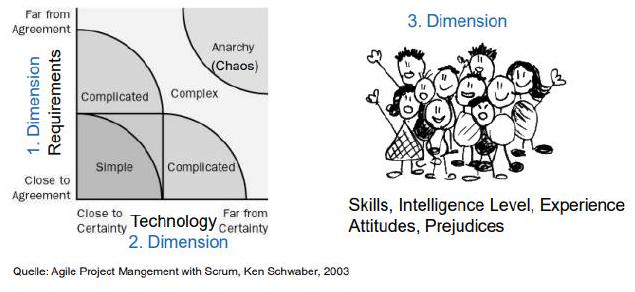
\includegraphics[width=\linewidth]{images/2024_12_29_0d1d7b5551ea1b4b41bdg-01}
\end{concept}



\begin{corollary}{Kernprozesse}

\begin{minipage}[t]{0.6\textwidth}
\begin{itemize}
  \item Anforderungserhebung
  \item Systemdesign/technische Konzeption
  \item Implementierung
  \item Softwaretest
  \item Softwareeinführung
  \item Wartung/Pflege
\end{itemize}
\end{minipage}
\begin{minipage}[t]{0.38\textwidth}
\textbf{\textcolor{frog}{Unterstützungsprozesse}}
\begin{itemize}
  \item Projektmanagement
  \item Qualitätsmanagement
  \item Risikomanagement 
\end{itemize}
\end{minipage}
\end{corollary}

\begin{concept}{Modelle in der Softwareentwicklung} 
\begin{itemize}
    \item Software ist selbst ein Modell der Realität
    \item Anforderungsmodelle beschreiben das Problem
    \item Architektur-/Entwurfsmodelle beschreiben die Lösung
    \item Testmodelle beschreiben korrektes Verhalten
\end{itemize}
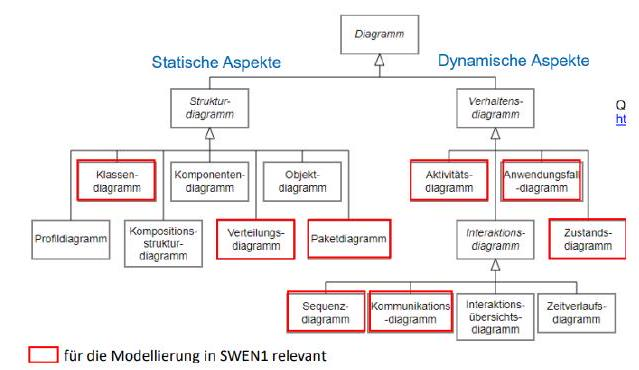
\includegraphics[width=\linewidth]{images/2024_12_29_0d1d7b5551ea1b4b41bdg-01(1)}
\end{concept}


\begin{formula}{Code and Fix}

Codierung und Korrektur im Wechsel

\begin{minipage}[t]{0.5\textwidth}
    Vorteile:
    \begin{itemize}
        \item Schnell und agil
        \item Einfach am Anfang
    \end{itemize}
\end{minipage}
\begin{minipage}[t]{0.5\textwidth}
    Nachteile:
    \begin{itemize}
        \item Schlecht planbar
        \item Schwer wartbar
        \item Änderungen aufwändig
    \end{itemize}
\end{minipage}
\end{formula}

\begin{formula}{Wasserfallmodell}

Sequentielle Phasen mit definierten Ergebnisdokumenten

\begin{minipage}[t]{0.5\textwidth}
    Vorteile:
    \begin{itemize}
        \item Gut planbar
        \item Klare Aufteilung in Phasen
        \item Definierte Meilensteine
    \end{itemize}
\end{minipage}
\begin{minipage}[t]{0.5\textwidth}
    Nachteile:
    \begin{itemize}
        \item Schlechtes Risikomanagement
        \item Spätes Kundenfeedback
        \item Unflexibel bei Änderungen
        \item Anforderungen nie vollständig zu Beginn bekannt
    \end{itemize}
\end{minipage}
\end{formula}

\begin{formula}{Iterativ-inkrementelle Modelle}

Schrittweise Entwicklung in geplanten Iterationen

\begin{minipage}[t]{0.4\textwidth}
Vorteile:
    \begin{itemize}
        \item Flexibles Modell
        \item Gutes Risikomanagement
        \item Frühe Einsetzbarkeit
        \item Kontinuierliches Kundenfeedback
    \end{itemize}
\end{minipage}
\begin{minipage}[t]{0.6\textwidth}
    Nachteile:
    \begin{itemize}
        \item Planung upfront hat Grenzen
        \item Höherer Koordinationsaufwand
    \end{itemize}
    Basis für agile Entwicklung:
    \begin{itemize}
        \item Fokus auf funktionierender Software
        \item Kurze Iterationen
        \item Enge Kundeneinbindung
    \end{itemize}
\end{minipage}

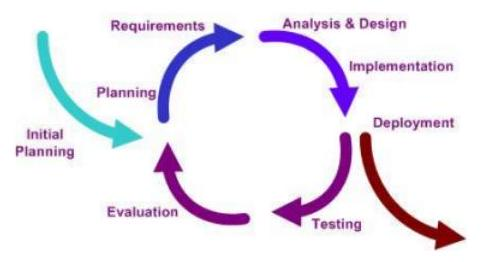
\includegraphics[width=0.8\linewidth]{images/2024_12_29_0d1d7b5551ea1b4b41bdg-02(1)}
\end{formula}


\begin{concept}{Charakteristiken iterativ-inkrementeller Prozesse}
\begin{itemize}
    \item Projekt-Abwicklung in Iterationen (Mini-Projekte)
    \item Inkrementelle Entwicklung (Stück für Stück)
    \item Risiko-getriebene Iterationsziele
    \item Reviews und Learnings nach jeder Iteration
    \item Demming-Cycle: Plan, Do, Check, Act
\end{itemize}
\end{concept}

\begin{example2}{Typische Prüfungsaufgabe: Prozessmodelle vergleichen}\\
    \small
Vergleichen Sie das Wasserfallmodell mit einem iterativ-inkrementellen Ansatz anhand folgender Kriterien:

Umgang mit sich ändernden Anforderungen, Risikomanagement, Planbarkeit, Kundeneinbindung
\vspace{1mm}\\
Musterlösung:
\begin{itemize}
    \item Wasserfall:
    \begin{itemize}
        \item Änderungen schwierig zu integrieren
        \item Risiken erst spät erkennbar
        \item Gut planbar durch feste Phasen
        \item Kunde hauptsächlich am Anfang und Ende involviert
    \end{itemize}
    \item Iterativ-inkrementell:
    \begin{itemize}
        \item Flexibel bei Änderungen
        \item Frühes Erkennen von Risiken
        \item Planung pro Iteration
        \item Kontinuierliches Kundenfeedback
    \end{itemize}
\end{itemize}
\end{example2}

\begin{definition}{Begriffe}
  \begin{itemize}
    \item Warum wird modelliert: Um Analyse- und Designentwürfe zu diskutieren, abstimmen und zu dokumentieren bzw. zu kommunizieren.
    \item Modell: Ein Modell ist ein konkretes oder gedankliches Abbild eines vorhanden Gebildes oder Vorbild für ein zu schaffendes Gebilde (hier Softwareprodukt).
    \item Original: Das Original ist das abgebildete oder zu schaffende Gebilde.
    \item Modellierung: Modellierung gehört zum Fundament des Software Engineerings
  \end{itemize}
\end{definition}

\subsubsection{Modellierung}

\begin{definition}{Modellierung in der Softwareentwicklung}
\begin{itemize}
    \item Modelle als Abstraktionen: Anforderungen, Architekturen, Testfälle.
    \item Einsatz von UML: Skizzen, detaillierte Blueprints, vollständige Spezifikationen.
    \item Zweck:
    \begin{itemize}
        \item Verstehen eines Gebildes
        \item Kommunizieren über ein Gebilde
        \item Gedankliches Hilfsmittel zum Gestalten, Bewerten, Kritisieren
        \item Spezifikation von Anforderungen
        \item Durchführung von Experimenten
    \end{itemize}
\end{itemize}
\end{definition}


\begin{KR}{Modellierungsumfang bestimmen}
Der benötigte Modellierungsumfang hängt ab von:
\begin{itemize}
    \item Komplexität der Problemstellung
    \item Anzahl beteiligter Stakeholder
    \item Kritikalität des Systems
    \item Domänenspezifische Anforderungen
    \item Analogie: Planung einer Hundehütte vs. Haus vs. Wolkenkratzer
\end{itemize}
\end{KR}

\begin{example2}{Prüfungsfrage zur Modellierung}\\
Erklären Sie anhand eines selbst gewählten Beispiels, warum der Modellierungsaufwand je nach Projekt stark variieren kann. Nennen Sie mindestens drei Faktoren, die den Modellierungsumfang beeinflussen.
\vspace{3mm}\\
Mögliche Antwort:
\begin{itemize}
    \item Beispiel: Entwicklung einer Smartphone-App vs. Medizinisches Gerät
    \item Faktoren:
    \begin{itemize}
        \item Komplexität der Domäne
        \item Regulatorische Anforderungen
        \item Anzahl beteiligter Stakeholder
        \item Sicherheitsanforderungen
    \end{itemize}
\end{itemize}
\end{example2}

\begin{definition}{Unified Modeling Language (UML)}
Standardsprache für grafische Modellierung:
\begin{itemize}
    \item \textbf{Einsatz als:}
    \begin{itemize}
        \item Sketch: Informelle Kommunikation und Verständnis
        \item Blueprint: Detaillierte Design-Spezifikation
        \item Programming Language: Ausführbare Modellierung
    \end{itemize}
    \item \textbf{Vorteile:}
    \begin{itemize}
        \item Standardisierte Notation
        \item Verschiedene Abstraktionsebenen
        \item Unterstützung des gesamten Entwicklungszyklus
    \end{itemize}
\end{itemize}
%todo: add UML diagram types overview
\end{definition}

